\subsection{Упражнение 1}

Убедимся, что analyze1 требует времени пропорционально n^3, а analyze2 пропорционален n^2 c помощью команды %timeit.

\begin{lstlisting}[language=Python]
import numpy as np
PI2 = np.pi * 2
def analyze1(ys, fs, ts):
    args = np.outer(ts, fs)
    M = np.cos(PI2 * args)
    amps = np.linalg.solve(M, ys)
    return amps
def analyze2(ys, fs, ts):
    args = np.outer(ts, fs)
    M = np.cos(PI2 * args)
    amps = M.dot(ys) / 2
    return amps
\end{lstlisting}

Возьмём размеры массива как степени 2.

\begin{lstlisting}[language=Python]
ns = 2 ** np.arange(5,10)
\end{lstlisting}

\begin{lstlisting}[language=Python]
best_analyze1 = []
for n in ns:
    ts = (0.5 + np.arange(n)) / n
    freqs = (0.5 + np.arange(n)) / 2
    ys = wave.ys[:n]
    best =  %timeit -r1 -o analyze1(ys,freqs,ts)
    best_analyze1.append(best.best)
best_analyze2 = []
for n in ns:
    ts = (0.5 + np.arange(n)) / n
    freqs = (0.5 + np.arange(n)) / 2
    ys = wave.ys[:n]
    best =  %timeit -r1 -o analyze2(ys,freqs,ts)
    best_analyze2.append(best.best)
best_dct = []
for n in ns:
    ys = wave.ys[:n]
    best =  %timeit -r1 -o scipy.fftpack.dct(ys, type=3)
    best_dct.append(best.best)
plt.plot(ns, best_analyze1, label='analyze1')
plt.plot(ns, best_analyze2, label='analyze2')
plt.plot(ns, best_dct, label='fftpack.dct')
loglog = dict(xscale='log', yscale='log')
decorate(xlabel='Wave length (N)', ylabel='Time (s)', **loglog)
\end{lstlisting}

\begin{figure}[H]
	\begin{center}
		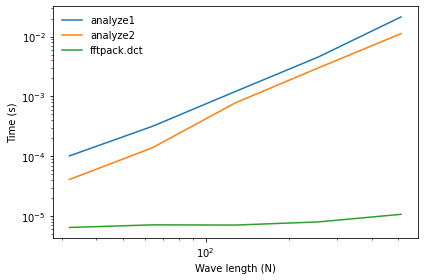
\includegraphics[scale=1]{fig/lab06/lab06_1.png}
		\caption{Время работы различных методов ДКП}
	\end{center}
\end{figure}

Не смотря на теоритическое время исполнения, время analyze1 получилсось пропорциональным  n2 .

\subsection{Упражнение 2}

Реализуем алгоритм ДКП и применим его для записи звуков или речи.

Возьмем звук пианино из первой лабораторной работы

\begin{lstlisting}[language=Python]
if not os.path.exists('jcveliz__violin-origional.wav'):
    !wget https://github.com/Eugenepolyt/telecomunaction/raw/main/jcveliz__violin-origional.wav
\end{lstlisting}

Выделим сегмент:

\begin{lstlisting}[language=Python]
segment = wave.segment(start = 1.2,duration = 0.5)
segment.normalize()
segment.make_audio()
\end{lstlisting}

DCT график для полученного сегмента

\begin{lstlisting}[language=Python]
dct = segment.make_dct()
dct.plot(high = 5000)
\end{lstlisting}


\begin{figure}[H]
	\begin{center}
		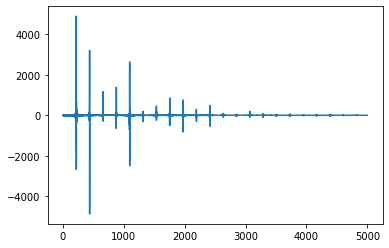
\includegraphics[scale=1]{fig/lab06/lab06_2.png}
		\caption{DCT график}
	\end{center}
\end{figure}

Следующая функция принимает dct и устанавливает все элементы ниже порога "trash" в ноль

\begin{lstlisting}[language=Python]
def compress(dct, thresh=1):
    count = 0
    for i, amp in enumerate(dct.amps):
        if np.abs(amp) < thresh:
            dct.hs[i] = 0
            count += 1
            
    n = len(dct.amps)
    print(count, n, 100 * count / n, sep='\t')
\end{lstlisting}

Применим функцию для нашего сегмента

\begin{lstlisting}[language=Python]
seg_dct = segment.make_dct()
compress(seg_dct, thresh=100)
seg_dct.plot(high=4000)
\end{lstlisting}
\begin{figure}[H]
	\begin{center}
		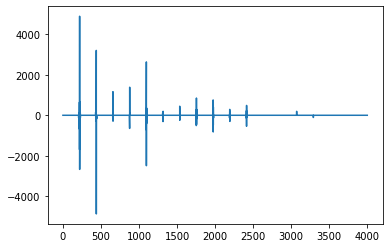
\includegraphics[scale=1]{fig/lab06/lab06_3.png}
		\caption{DCT после фильтрации}
	\end{center}
\end{figure}


\subsection{Управжнение 3}

В блокноте phase.ipynb взять другой сегмент звука и повторить эксперименты.

\begin{lstlisting}[language=Python]
from thinkdsp import SawtoothSignal
signal = SawtoothSignal(freq=500, offset=0)
wave.segment(start=0.02,duration=0.01).plot()
decorate(xlabel='Time (s)')
\end{lstlisting}
\begin{figure}[H]
	\begin{center}
		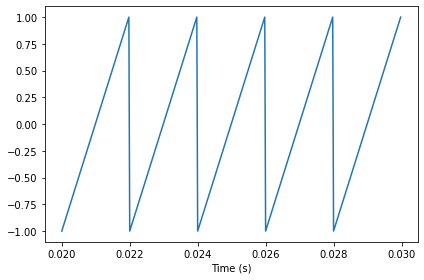
\includegraphics[scale=1]{fig/lab06/lab06_4.png}
		\caption{График сегмента}
	\end{center}
\end{figure}

\begin{lstlisting}[language=Python]
spectrum = wave.make_spectrum()
spectrum.plot()
decorate(xlabel='Frequency (Hz)',
         ylabel='Amplitude')
\end{lstlisting}

\begin{figure}[H]
	\begin{center}
		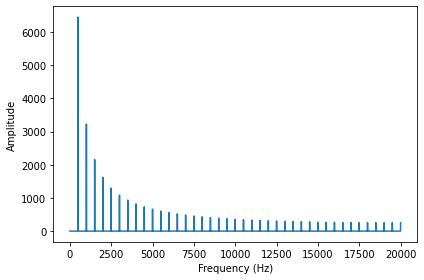
\includegraphics[scale=1]{fig/lab06/lab06_5.png}
		\caption{Спектр сегмента}
	\end{center}
\end{figure}

\begin{lstlisting}[language=Python]
def plot_angle(spectrum, thresh=1):
    angles = spectrum.angles
    angles[spectrum.amps < thresh] = np.nan
    plt.plot(spectrum.fs, angles, 'x')
    decorate(xlabel='Frequency (Hz)', 
             ylabel='Phase (radian)')
plot_angle(spectrum, thresh=0)
plot_angle(spectrum, thresh=1)
def plot_three(spectrum, thresh=1):
    """Plot amplitude, phase, and waveform.
    
    spectrum: Spectrum object
    thresh: threshold passed to plot_angle
    """
    plt.figure(figsize=(10, 4))
    plt.subplot(1,3,1)
    spectrum.plot()
    plt.subplot(1,3,2)
    plot_angle(spectrum, thresh=thresh)
    plt.subplot(1,3,3)
    wave = spectrum.make_wave()
    wave.unbias()
    wave.normalize()
    wave.segment(duration=0.01).plot()
    display(wave.make_audio())
\end{lstlisting}

\begin{lstlisting}[language=Python]
plot_three(spectrum)
\end{lstlisting}
\begin{figure}[H]
	\begin{center}
		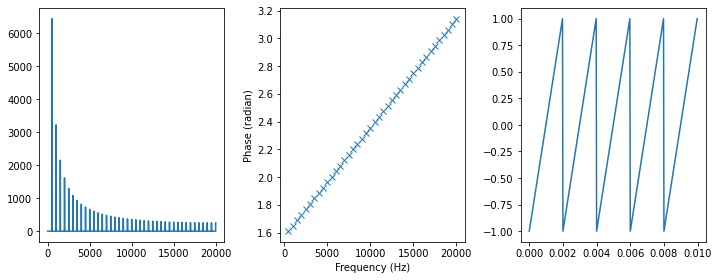
\includegraphics[scale=0.66]{fig/lab06/lab06_6.png}
		\caption{Результат работы функции}
	\end{center}
\end{figure}

\begin{lstlisting}[language=Python]
def zero_angle(spectrum):
    res = spectrum.copy()
    res.hs = res.amps
    return res
spectrum2 = zero_angle(spectrum)
plot_three(spectrum2)
\end{lstlisting}
\begin{figure}[H]
	\begin{center}
		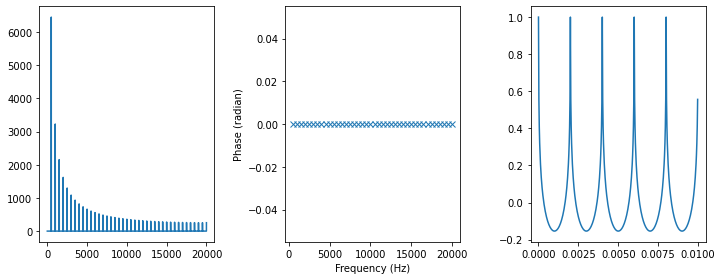
\includegraphics[scale=0.66]{fig/lab06/lab06_7.png}
		\caption{Результат работы функции}
	\end{center}
\end{figure}

\begin{lstlisting}[language=Python]
def rotate_angle(spectrum, offset):
    res = spectrum.copy()
    res.hs *= np.exp(1j * offset)
    return res
\end{lstlisting}
\begin{figure}[H]
	\begin{center}
		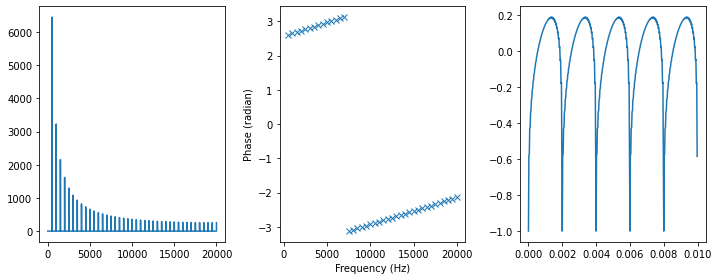
\includegraphics[scale=0.66]{fig/lab06/lab06_8.png}
		\caption{Результат работы функции}
	\end{center}
\end{figure}


\begin{lstlisting}[language=Python]
PI2 = np.pi * 2

def random_angle(spectrum):
    res = spectrum.copy()
    angles = np.random.uniform(0, PI2, len(spectrum))
    res.hs *= np.exp(1j * angles)
    return res
spectrum4 = random_angle(spectrum)
plot_three(spectrum4)
\end{lstlisting}
\begin{figure}[H]
	\begin{center}
		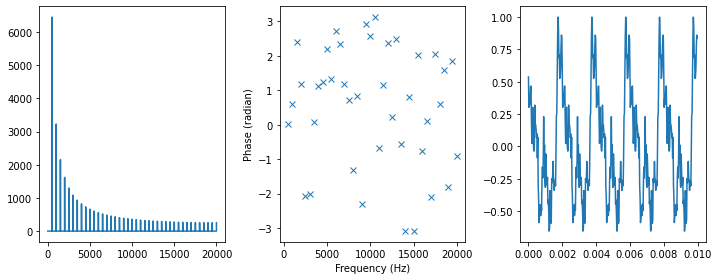
\includegraphics[scale=0.66]{fig/lab06/lab06_9.png}
		\caption{Результат работы функции}
	\end{center}
\end{figure}

Звук звучит также, как первоначальный, возьмем другой звук. 

\begin{lstlisting}[language=Python]
if not os.path.exists('120994__thirsk__120-oboe.wav'):
    !wget https://github.com/AllenDowney/ThinkDSP/raw/master/code/120994__thirsk__120-oboe.wav
from thinkdsp import read_wave
wave = read_wave('120994__thirsk__120-oboe.wav')
wave.make_audio()
segment = wave.segment(start=0.2, duration=0.5)
spectrum = segment.make_spectrum()
\end{lstlisting}

\begin{lstlisting}[language=Python]
plot_three(spectrum)
\end{lstlisting}
\begin{figure}[H]
	\begin{center}
		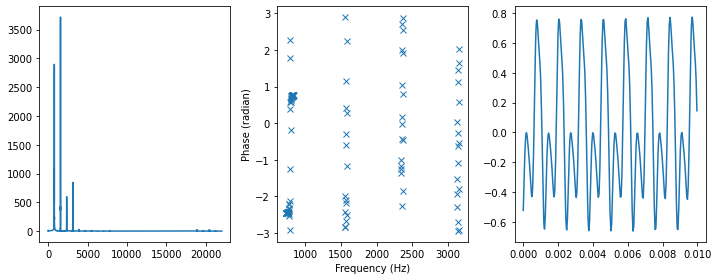
\includegraphics[scale=0.66]{fig/lab06/lab06_10.png}
		\caption{Результат работы функции}
	\end{center}
\end{figure}

\begin{lstlisting}[language=Python]
spectrum2 = zero_angle(spectrum)
plot_three(spectrum2, thresh=50)
\end{lstlisting}
\begin{figure}[H]
	\begin{center}
		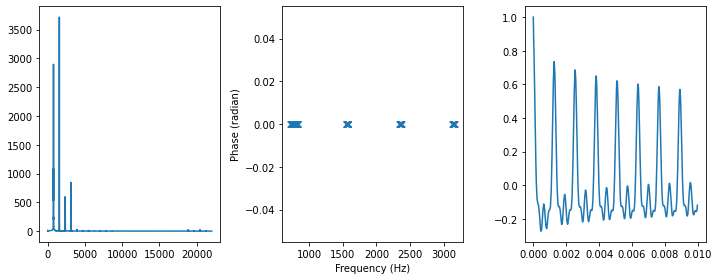
\includegraphics[scale=0.66]{fig/lab06/lab06_11.png}
		\caption{Результат работы функции}
	\end{center}
\end{figure}

Звук стал более глухой


\begin{lstlisting}[language=Python]
spectrum3 = rotate_angle(spectrum, 1)
plot_three(spectrum3, thresh=50)
\end{lstlisting}
\begin{figure}[H]
	\begin{center}
		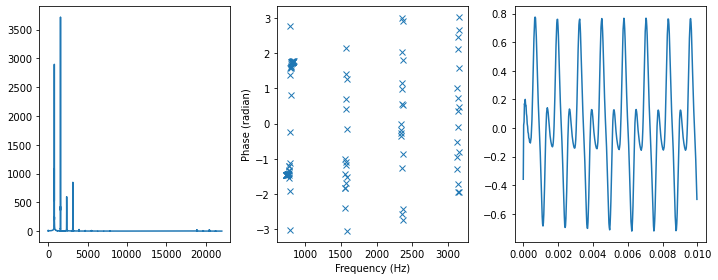
\includegraphics[scale=0.66]{fig/lab06/lab06_12.png}
		\caption{Результат работы функции}
	\end{center}
\end{figure}


\begin{lstlisting}[language=Python]
spectrum4 = random_angle(spectrum)
plot_three(spectrum4)
\end{lstlisting}
\begin{figure}[H]
	\begin{center}
		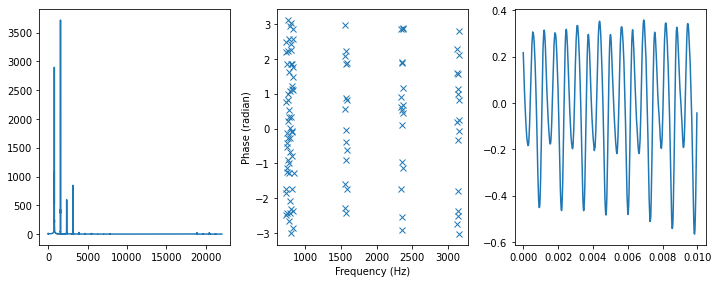
\includegraphics[scale=0.66]{fig/lab06/lab06_13.png}
		\caption{Результат работы функции}
	\end{center}
\end{figure}

В данном случае звук уже отличается от изначального, но не сильно. Мы не слышим особо изменения в фазовой структуре, если гармоническая структура не изменялась.

\subsection{Вывод}
В данной лабораторной работе был рассмотрен ДКП , который применяется в различных форматах сжатия музыки. С помощью ДКП были рассмотрены свойства звуков с разной структурой
